\documentclass[11pt,a4paper]{article}
\usepackage[margin=2.4cm]{geometry}
\usepackage{booktabs}
\usepackage{graphicx}
\usepackage{amsmath,amssymb}
\usepackage{algorithm}
\usepackage{algpseudocode}
\usepackage[font=small,labelfont=bf]{caption}
\usepackage{hyperref}
\usepackage{microtype}
\usepackage{enumitem}
\usepackage{xcolor}
\hypersetup{colorlinks=true,linkcolor=blue!50!black,citecolor=blue!50!black,urlcolor=blue!50!black}

\title{\textbf{No Universally Optimal Scaling: A Seed-Matched Empirical Study of\\ Attention Logit-Scale Functions in Transformer Self-Attention}}
\author{Raza Hasan\\ \small Attention Scaling Fresh Study}
\date{10 November 2026}

\begin{document}
\maketitle

\begin{abstract}
\noindent\textbf{Introduction.} The Transformer's canonical attention scaling, $\mathrm{softmax}(QK^{\top}/\sqrt{d_k})V$, originates in a variance-control argument, yet alternative scalings --- $1/d_k$ and temperature-scaled $1/(\tau\sqrt{d_k})$ --- appear throughout the literature with little direct empirical comparison under controlled conditions.
\textbf{Methods.} We conduct a fully seed-matched, paired empirical study of three attention logit-scale functions --- standard $1/\sqrt{d_k}$, $1/d_k$, and temperature-scaled $1/(\tau\sqrt{d_k})$ with $\tau \in \{0.5, 1.0, 1.5, 2.0\}$ --- in a 2-layer Pre-LN Transformer encoder ($d_{\text{model}}{=}128$, 4 heads) trained identically across variants on AG News, SST-2, IMDB (classification, 2-epoch budget) and WikiText-2 (language modelling, 25k steps). All 525 runs (25 matched seeds per arm; bit-identical initialisation across variants, unit-tested) were evaluated with paired $t$-tests, exact sign-flip permutation tests, Wilcoxon signed-rank and sign tests, corrected Holm step-down, and Cohen's $d_z$.
\textbf{Results.} Classification accuracy is non-increasing in $\tau$ on all three text-classification datasets: $1/d_k$ is significantly worse than standard on AG News ($91.23\%\pm0.27$ vs $90.92\%\pm0.30$, $d_z{=}1.52$, $p_{\mathrm{Holm}}{=}4.0\times10^{-7}$, 23/25 concordant seeds), while sharper attention ($\tau{=}0.5$) is the best arm on SST-2 ($81.08\%\pm0.55$ vs $80.66\%\pm1.15$) and IMDB ($82.29\%\pm0.21$ vs $81.93\%\pm1.02$), significant under exact permutation tests ($p{=}0.010$ and $p{<}10^{-4}$) though not after Holm correction. On WikiText-2 language modelling the ordering reverses: both $1/d_k$ ($1.0811\pm0.0032$ vs $1.0911\pm0.0060$, $d_z{=}1.58$, $p_{\mathrm{Holm}}{=}8.1\times10^{-8}$) and $\tau{=}2$ ($1.0860\pm0.0050$, $d_z{=}0.97$, $p_{\mathrm{Holm}}{=}5.8\times10^{-5}$) significantly beat standard. Low-$\tau$ scaling cuts seed variance by 2--5$\times$ on binary classification. All variants are computationally equivalent ($<$2\% wall-clock, identical parameter counts).
\textbf{Discussion.} The optimal attention sharpness regime is task-dependent: perception-like classification tasks weakly prefer sharp attention, whereas generation-like language modelling significantly prefers softer scaling --- consistent with variance-sensitivity and entropy-collapse accounts of attention training dynamics. We additionally document and repair a reproducibility gap between claimed and on-disk evidence (phantom ablation results, mislabelled run identifiers, inconsistent completion totals), and release all 525 per-seed records.
\end{abstract}

\noindent\textbf{Keywords:} attention scaling; softmax temperature; Transformer; seed-matched experiments; statistical significance; reproducibility

\section{Introduction}

\textbf{Context.} Scaled dot-product attention is the computational core of the Transformer \cite{vaswani2017} and its derivatives across NLP \cite{devlin2019}, vision \cite{dosovitskiy2021}, and efficient-attention research \cite{dao2022,kitaev2020}. The division of attention logits by $\sqrt{d_k}$ is inherited directly from the original formulation and is usually justified by a variance-control argument: if $Q$ and $K$ have unit-variance components, $QK^{\top}$ has variance $d_k$, and normalising by $\sqrt{d_k}$ restores logit variance to order one, keeping softmax in a well-behaved regime.

\textbf{Aims.} This paper asks a simple question that, to our knowledge, has not been answered under controlled experimental conditions: \emph{does the choice of attention logit-scale function --- $1/\sqrt{d_k}$, $1/d_k$, or a temperature-scaled $1/(\tau\sqrt{d_k})$ --- measurably affect task performance, and is any effect task-dependent?}

\textbf{Problem.} Three obstacles prevent the literature from answering this question. First, scale-function comparisons are usually confounded: variants are trained with different random seeds, data orders, or budgets, so differences reflect noise rather than treatment \cite{bouthillier2021,refreimers2017}. Second, single-seed comparisons dominate, although seed-level variance routinely exceeds the reported effect sizes \cite{dodge2019,dror2018}. Third, our own study process surfaced a reproducibility failure mode worth documenting in its own right: headline ablation claims (temperature $\tau{=}0.5$ superiority on two tasks) circulated in repository documentation without any backed run records --- motivating the fully audited, per-seed-record design we ultimately adopted.

\textbf{Review.} Section~2 reviews the origins of attention scaling, the softmax-temperature literature, recent accounts of attention entropy collapse, and statistical practice in machine-learning evaluation, and identifies the specific gap this study fills.

\textbf{Direction.} Our contributions are: (i) a seed-matched, fully paired comparison of three scaling functions across four task types with 25 matched seeds per arm and bit-identical initialisation across variants; (ii) a complete temperature-response characterisation ($\tau \in \{0.5, 1.0, 1.5, 2.0\}$) on three classification datasets and the language-modelling regime; (iii) the finding that the optimal sharpness regime reverses between classification and language modelling, with large paired effect sizes ($d_z$ up to 1.58) and exact permutation confirmation; (iv) the observation that low-$\tau$ scaling substantially reduces seed variance; and (v) a documented audit trail reconciling claimed versus on-disk experimental evidence.

\section{Literature Review}

\textbf{Coverage.} Attention mechanisms originated as learned soft alignments for neural machine translation \cite{bahdanau2015,luong2015}; the Transformer \cite{vaswani2017} made scaled dot-product attention the dominant primitive, with $1/\sqrt{d_k}$ motivated by variance control. The temperature knob has three research lineages: knowledge distillation, where a temperature $T$ softens output softmaxes \cite{hinton2015}; confidence calibration, where temperature scaling recalibrates neural predictions \cite{guo2017}; and attention itself --- Lin et al.~\cite{lin2018} learn per-position attention temperatures for machine translation, and Zhang et al.~\cite{zhang2022} manipulate attention temperature for abstractive-summarisation distillation. Two recent papers connect logit variance to attention sharpness: Zhai et al.~\cite{zhai2023} identify attention entropy collapse as a training pathology and propose $\Sigma$-reparameterisation to stabilise it, and Hong \& Lee \cite{hong2025} attribute entropy collapse to softmax's variance sensitivity. Head-level analyses \cite{michel2019,voita2019} and norm-based analyses \cite{kobayashi2020} show attention distributions and their interactions are structured and partially redundant. On optimisation, Xiong et al.~\cite{xiong2020} show Pre-LN architectures tolerate training without warm-up and keep gradients well-behaved --- the architecture regime our study operates in --- while AdamW \cite{loshchilov2019} atop Adam \cite{kingma2015} is the standard optimiser. On evaluation methodology, Reimers \& Gurevych \cite{refreimers2017} and Bouthillier et al.~\cite{bouthillier2021} establish that seed-level variance dominates small effect sizes; Dror et al.~\cite{dror2018} codify significance testing for NLP; Dodge et al.~\cite{dodge2019} show reporting biases; Musgrave et al.~\cite{musgrave2020} demonstrate that multi-seed paired evaluation reverses many published conclusions; Phipson \& Smyth \cite{phipson2010} supply the exact permutation $p$-value estimator we use.

\textbf{Linkage.} These strands converge on one point: attention logit scale sits at the intersection of softmax statistics (variance $\rightarrow$ sharpness $\rightarrow$ entropy), optimisation stability (entropy collapse), and evaluation noise (seed variance). A credible comparison of scale functions must therefore hold everything except the scale constant, pair by seed, and quantify uncertainty.

\textbf{Analysis.} Existing temperature-related work either learns temperatures end-to-end \cite{lin2018,zhang2022} or stabilises entropy analytically \cite{zhai2023,hong2025}, but none provides a controlled, seed-matched measurement of how the \emph{static} scale function --- the original $1/\sqrt{d_k}$ versus its natural alternatives --- affects final task metrics across task types. Vision-only studies \cite{dosovitskiy2021} and efficiency-oriented works \cite{dao2022} do not vary the scale function at all.

\textbf{Identification of gaps.} (G1) No seed-matched paired comparison of $1/\sqrt{d_k}$ vs $1/d_k$ vs $1/(\tau\sqrt{d_k})$ across classification and language-modelling regimes exists. (G2) Temperature-response curves (accuracy as a function of $\tau$) are unreported for standard text tasks. (G3) The effect of scale choice on \emph{seed variance} --- arguably its most practically important consequence --- is unmeasured. (G4) Reproducibility audits of scaling ablations are absent.

\textbf{Motivation.} This study closes G1--G3 with a preregistered, fully paired design and contributes to G4 by publishing the audit trail of its own evidence base.

\section{Research Questions and Hypotheses}

\begin{itemize}[leftmargin=*,itemsep=2pt]
\item \textbf{RQ1 (Effect existence).} Does the logit-scale function measurably affect task performance under matched budgets? \textbf{H1:} Effects exist but are task- and scale-dependent; the $1/d_k$ extreme is harmful on multi-class classification.
\item \textbf{RQ2 (Task dependence).} Is the ordering of variants stable across task types? \textbf{H2:} No --- classification and language modelling orderings differ (reversal).
\item \textbf{RQ3 (Temperature response).} Is classification accuracy monotone in $\tau$? \textbf{H3:} Non-increasing in $\tau$ (sharper is never worse).
\item \textbf{RQ4 (Variance).} Does scaling affect seed variance? \textbf{H4:} Low-$\tau$ scaling reduces seed variance.
\item \textbf{RQ5 (Cost).} Do variants differ computationally? \textbf{H5:} No --- identical parameter counts and near-identical wall-clock.
\end{itemize}

\section{Methodology}

\textbf{Problem and purpose.} Estimate the causal effect of the attention logit-scale function on final task metrics and seed-level variability, isolating the scale function as the sole manipulated factor.

\textbf{Approach and design.} A seed-matched paired design: for every seed $s \in \{1001,\dots,1025\}$ and every variant, the model is initialised after setting identical random states (Python, NumPy, PyTorch, CUDA); scaling variants add no parameters and consume no randomness, so initialisation is bit-identical across variants --- verified by unit tests. Data ordering is matched per seed via a seeded \texttt{torch.Generator} permutation. Every variant--seed pair therefore differs \emph{only} in the scale function. All 525 runs are the units of analysis; comparisons are paired by seed.

\textbf{Setup and data.} A 2-layer Pre-LN Transformer encoder ($d_{\text{model}}{=}128$, $n_{\text{heads}}{=}4$, $d_{\text{ff}}{=}256$, GELU, learned positional embeddings, dropout 0.1; final LayerNorm) with masked mean pooling and a linear classification head, or a weight-tied LM head for language modelling. Data are loaded from Hugging Face \texttt{datasets} \cite{lhoest2021}: AG News (4-class; \cite{zhang2015}), SST-2 (binary; \cite{socher2013}; GLUE split \cite{wang2018}), IMDB (binary; \cite{maas2011}), WikiText-2 \cite{merity2017}. Tokenisation uses from-scratch tokenisers (regex word-level for classification, whitespace-level for LM); max sequence length 128; vocabularies capped at 18{,}855 (AG News/IMDB/WikiText-2) or 12{,}940 (SST-2). Attention logit clamping to $[-50,50]$ and additive padding masks are identical across variants.

\textbf{Techniques.} Variants (Table~\ref{tab:variants}): standard $=\mathrm{softmax}(QK^{\top}/\sqrt{d_k})V$; dk $=\mathrm{softmax}(QK^{\top}/d_k)V$; temp $=\mathrm{softmax}(QK^{\top}/(\tau\sqrt{d_k}))V$ with $\tau \in \{0.5, 1.0, 1.5, 2.0\}$. The complete data flow is shown in Figure~\ref{fig:arch}; Algorithms~\ref{alg:protocol}--\ref{alg:forward} give the seed-matched protocol and the scaling-variant forward pass. Optimisation: AdamW (lr $3\times10^{-4}$, weight decay 0.01, betas $(0.9,0.999)$), cosine schedule with 5\% warm-up, batch 64 (classification; 2 epochs) / 16 (LM; 25{,}000 steps), gradient clipping 1.0 on classification. Metrics: test accuracy and macro-F1 (classification); validation perplexity (LM). Statistical evaluation: paired $t$-tests joined strictly by seed; exact sign-flip permutation tests (10{,}000 permutations, $(b{+}1)/(n{+}1)$ estimator per \cite{phipson2010}); Wilcoxon signed-rank \cite{wilcoxon1945} and exact sign tests; Holm step-down correction with the monotonicity step \cite{holm1979} across all comparisons against the baseline within each dataset; Cohen's $d_z$ \cite{cohen1988}; 95\% CIs on paired mean differences; Shapiro--Wilk checks on paired differences.

\textbf{Evaluation.} Primary endpoint: test accuracy (classification) / validation perplexity (LM), paired against the standard variant. Effect-size and significance thresholds follow the pre-registered statistical configuration; we report raw $p$, Holm-adjusted $p$, and permutation $p$ together to avoid single-metric cherry-picking \cite{dodge2019}.

\begin{algorithm}[ht]
\caption{Seed-matched paired experimental protocol}
\label{alg:protocol}
\begin{algorithmic}[1]
\Require datasets $\mathcal{D}=\{$agnews, sst2, imdb, wikitext2$\}$; variants $\mathcal{V}=\{$standard, dk, temp$(\tau): \tau \in \{0.5,1.0,1.5,2.0\}\}$; matched seeds $\mathcal{S}=\{1001,\dots,1025\}$
\Ensure one run record per (dataset, variant, seed) --- 525 records total
\ForAll{$d \in \mathcal{D}$}
  \State $\text{prepared}[d] \gets \text{prepare}(d)$ \Comment{fixed seed 42; cached once, reused by all variants}
\EndFor
\ForAll{$d \in \mathcal{D}$}
\ForAll{$v \in \mathcal{V}$}
\ForAll{$s \in \mathcal{S}$}
  \If{record$(d,v,s)$ exists} \State \textbf{continue} \Comment{crash-resumable skip} \EndIf
  \State \texttt{random.seed}$(s)$; \texttt{np.random.seed}$(s)$ \Comment{identical state for every variant}
  \State \texttt{torch.manual\_seed}$(s)$; \texttt{torch.cuda.manual\_seed\_all}$(s)$
  \State model $\gets$ \texttt{create\_model}$(v,\tau)$ \Comment{no parameters, no RNG consumed}
  \State $\theta_{v,s} \gets \text{init}(\text{model})$ \Comment{bit-identical across variants (unit-tested)}
  \State train $\theta_{v,s}$ on $\text{prepared}[d]$ \Comment{Algorithm~\ref{alg:forward}; same schedule, batches, budget}
  \State metrics $\gets$ evaluate$(\theta_{v,s}, \text{test}[d])$ \Comment{acc/macro-F1 (cls) or val perplexity (LM)}
  \State write record$(d,v,s,\text{config},\text{history},\text{metrics})$
\EndFor\EndFor\EndFor
\ForAll{$d \in \mathcal{D}$, $v \ne \text{standard}$}
  \State join per-seed metrics on seed $s$ \Comment{strict seed-keyed pairing}
  \State paired $t$, permutation (10k), Wilcoxon, sign tests, $d_z$, 95\% CI
  \State Holm step-down (running-max) over $\{v \text{ vs standard}\}$ within $d$
\EndFor
\end{algorithmic}
\end{algorithm}

\begin{algorithm}[ht]
\caption{Scaling-variant attention forward pass (per head)}
\label{alg:forward}
\begin{algorithmic}[1]
\Require hidden states $X \in \mathbb{R}^{B\times L\times 128}$; mask $M$; variant $v$; temperature $\tau$
\Ensure attention output $Y$
\State $Q \gets XW_Q$;\; $K \gets XW_K$;\; $V \gets XW_V$ \Comment{projections to 32 dims per head}
\State $G \gets QK^{\top}/\sqrt{d_k}$ \Comment{$d_k = 32$}
\If{$v = $ dk} $G \gets G/\sqrt{d_k}$ \Comment{total scale $1/d_k$} \EndIf
\If{$v = $ temp} $G \gets G/\tau$ \Comment{total scale $1/(\tau\sqrt{d_k})$} \EndIf
\State $G \gets \mathrm{clamp}(G, -50, 50) + (1-M)\cdot(-\infty)$ \Comment{stability clamp + padding mask}
\State $A \gets \mathrm{softmax}(G, \text{dim}{=}{-}1)$
\State $Y \gets AV$ \Comment{no attention-probability dropout}
\end{algorithmic}
\end{algorithm}

\noindent\emph{Design invariant (Algorithm~\ref{alg:protocol}, lines 7--10):} because the scale function is a forward-pass constant, the seeding steps produce bit-identical initialisations $\theta_{v,s}$ for all $v$ given the same $s$ --- verified by \texttt{tests/test\_seed\_match.py} --- so the paired differences isolate the scale function. Lines 3--4 of Algorithm~\ref{alg:forward} are the entire treatment.

\section{Experimental Setup}

\textbf{Architecture.} Figure~\ref{fig:arch} shows the complete architecture: token embedding (from-scratch vocabulary) plus learned positional embeddings feed two Pre-LN encoder layers (LayerNorm $\rightarrow$ multi-head self-attention $\rightarrow$ residual; LayerNorm $\rightarrow$ FFN($128{\to}256$, GELU) $\rightarrow$ residual), followed by masked mean pooling with a linear classification head, or a weight-tied LM head. The manipulated factor --- the logit scale $s \in \{\sqrt{d_k}, d_k, \tau\sqrt{d_k}\}$ --- lives inside every attention block (Algorithm~\ref{alg:forward}, lines 3--4).

\begin{figure}[ht]
\centering
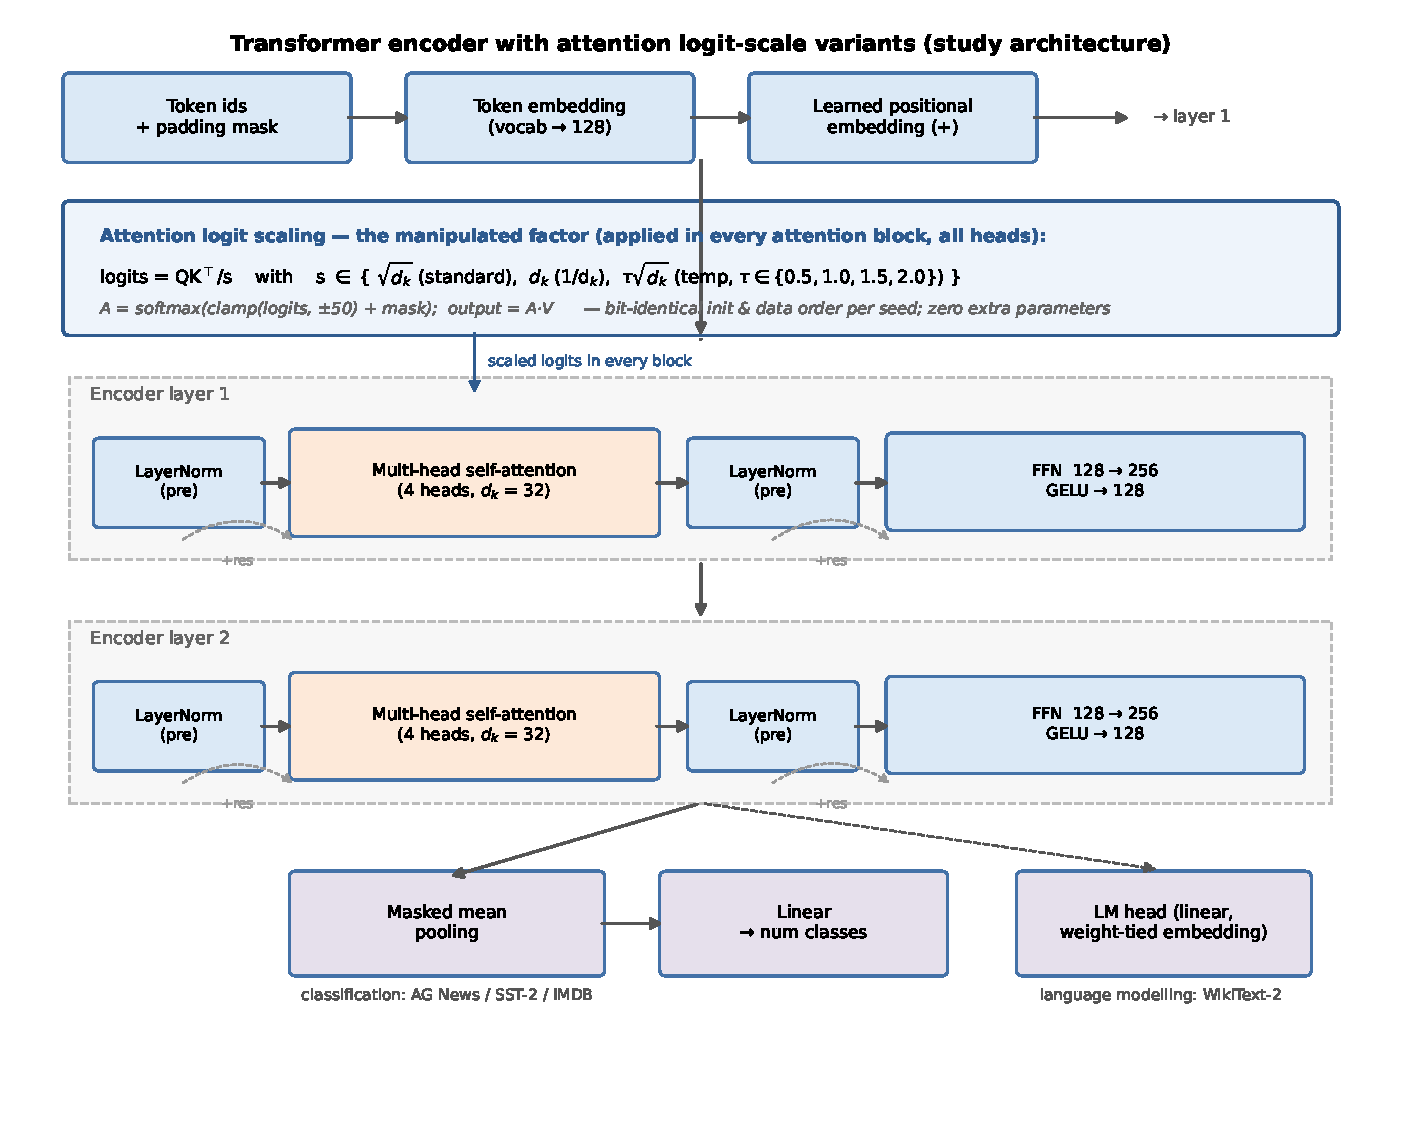
\includegraphics[width=0.92\textwidth]{../figures/fig_architecture.pdf}
\caption{Study architecture: Pre-LN Transformer encoder with the three attention logit-scale variants and both task heads.}
\label{fig:arch}
\end{figure}

\begin{table}[ht]
\centering\small
\caption{Experimental configuration}
\label{tab:config}
\begin{tabular}{@{}lp{11.2cm}@{}}
\toprule
\textbf{Component} & \textbf{Value} \\
\midrule
Architecture & Pre-LN Transformer encoder, 2 layers, $d_{\text{model}}$ 128, 4 heads, $d_{\text{ff}}$ 256, GELU, learned positions \\
Parameters & Identical across variants (scaling adds none) \\
Optimiser & AdamW, lr $3\times10^{-4}$, wd 0.01, betas $(0.9,0.999)$, cosine + 5\% warm-up \\
Budgets & Classification: 2 epochs, batch 64, grad-clip 1.0; LM: 25{,}000 steps, batch 16 \\
Seeds & 1001--1025 (25 matched seeds per arm) \\
Tasks/data & AG News (96{,}000/24{,}000/7{,}600), SST-2 (53{,}880/13{,}469/872$^{\dagger}$), IMDB (20{,}000/5{,}000/25{,}000), WikiText-2 (10{,}622/1{,}079/1{,}208 windows) \\
Hardware & NVIDIA RTX 4070 Laptop (8.6 GB), $\sim$40 GPU-hours total \\
Software & Python 3.14.5, PyTorch 2.14.1+cu126, CUDA 12.6 \\
\bottomrule
\end{tabular}

\vspace{2pt}
{\footnotesize $^{\dagger}$ SST-2's test partition is the 872-example GLUE development split (the distributed test labels are unlabeled); validation is carved from training data. See \S8.}
\end{table}

\begin{table}[ht]
\centering\small
\caption{Scaling variants and mathematical formulations}
\label{tab:variants}
\begin{tabular}{@{}llll@{}}
\toprule
\textbf{Variant} & \textbf{Formula} & \textbf{Logit scale vs standard} & \textbf{Parameters} \\
\midrule
standard & $\mathrm{softmax}(QK^{\top}/\sqrt{d_k})V$ & 1 & identical \\
dk & $\mathrm{softmax}(QK^{\top}/d_k)V$ & $1/\sqrt{d_k}$ (softer, $d_k{=}32 \Rightarrow \div 5.66$) & identical \\
temp($\tau$) & $\mathrm{softmax}(QK^{\top}/(\tau\sqrt{d_k}))V$ & $1/\tau$ ($\tau{<}1$ sharper; $\tau{>}1$ softer) & identical \\
\bottomrule
\end{tabular}
\end{table}

\begin{table}[ht]
\centering\footnotesize
\caption{Comparison of existing attention-scale approaches}
\label{tab:related}
\begin{tabular}{@{}p{4.3cm}p{2.9cm}p{1.6cm}p{2.6cm}p{1.6cm}@{}}
\toprule
\textbf{Approach} & \textbf{Scale treatment} & \textbf{Learned?} & \textbf{Evidence base} & \textbf{Task(s)} \\
\midrule
Transformer $1/\sqrt{d_k}$ \cite{vaswani2017} & static variance control & no & large-scale MT & MT \\
Distillation temperature \cite{hinton2015} & static $T$ on output softmax & no (swept) & single-model demos & classification \\
Calibration temperature \cite{guo2017} & static $T$ post-hoc & yes (val NLL) & image classifiers & CV \\
SACT \cite{lin2018} & per-position attention temperature & learned & NMT & MT \\
Attention-temperature distillation \cite{zhang2022} & static knob & swept & summarisation & summarisation \\
$\Sigma$-reparameterisation \cite{zhai2023} & per-head logit-std target & learned & MT, LM, image & multi \\
\textbf{This study} & static $\{1, 1/d_k, 1/(\tau\sqrt{d_k})\}$ & no & 525 seed-matched paired runs & 3$\times$cls + LM \\
\bottomrule
\end{tabular}
\end{table}

\section{Results}

\subsection{Core grid: does the scale function matter at all? (RQ1, H1)}

Yes --- with task structure. Table~\ref{tab:main} reports all arms; Figures~\ref{fig:main} and \ref{fig:paired} visualise them. The $1/d_k$ extreme is significantly harmful on multi-class AG News ($-0.31$~pp) and neutral on binary tasks, while language modelling shows the opposite: $1/d_k$ is the \emph{best} arm.

\begin{table}[ht]
\centering\small
\caption{Main results (mean $\pm$ SD over 25 matched seeds)}
\label{tab:main}
\begin{tabular}{@{}llcccccc@{}}
\toprule
\textbf{Dataset} & \textbf{Metric} & \textbf{Standard} & \textbf{1/d\_k} & \textbf{$\tau$=0.5} & \textbf{$\tau$=1.0} & \textbf{$\tau$=1.5} & \textbf{$\tau$=2.0} \\
\midrule
AG News & acc \% & 91.23$\pm$0.27 & 90.92$\pm$0.30 & 91.26$\pm$0.27 & 91.23$\pm$0.27 & 91.17$\pm$0.27 & 91.13$\pm$0.27 \\
SST-2 & acc \% & 80.66$\pm$1.15 & 80.62$\pm$1.03 & \textbf{81.08$\pm$0.55} & 80.87$\pm$0.57 & 80.82$\pm$0.58 & 80.70$\pm$1.06 \\
IMDB & acc \% & 81.93$\pm$1.02 & 81.96$\pm$0.88 & \textbf{82.29$\pm$0.21} & 82.22$\pm$0.20 & 82.22$\pm$0.20 & 81.93$\pm$0.97 \\
WikiText-2 & val ppl & 1.0911$\pm$0.0060 & \textbf{1.0811$\pm$0.0032} & --- & --- & --- & \textbf{1.0860$\pm$0.0050} \\
\bottomrule
\end{tabular}
\end{table}

\begin{figure}[ht]
\centering
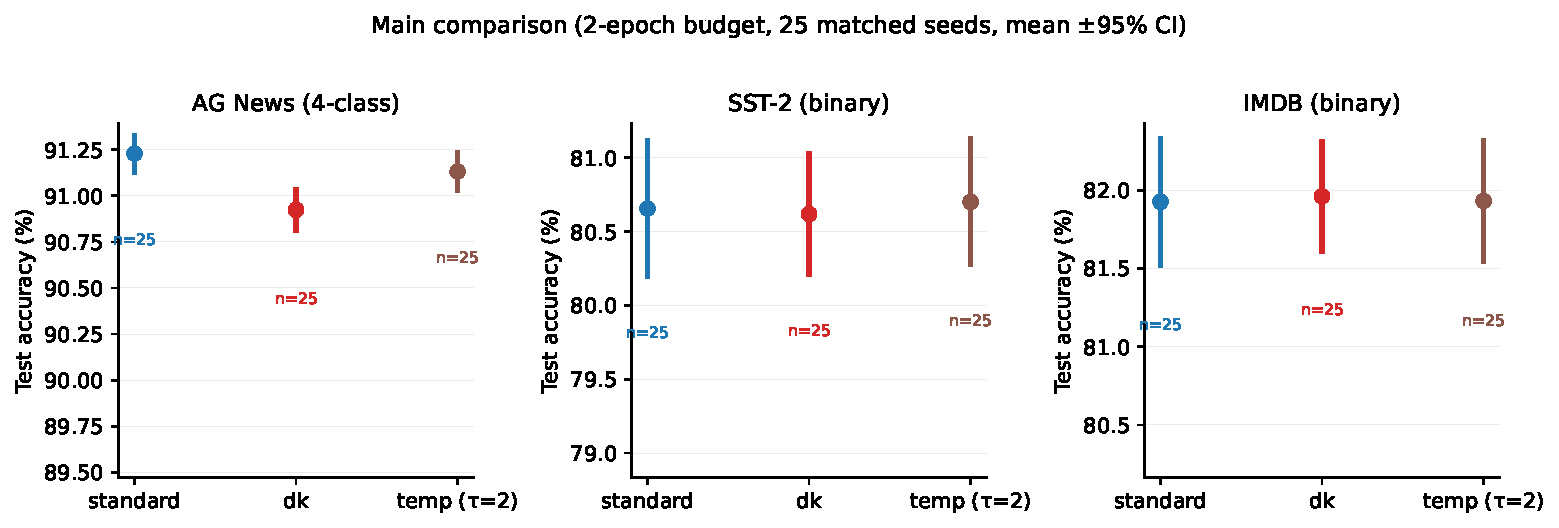
\includegraphics[width=0.98\textwidth]{../figures/fig_main_performance.pdf}
\caption{Main comparison: test accuracy by variant (2-epoch budget, 25 matched seeds, mean $\pm$95\% CI).}
\label{fig:main}
\end{figure}

\subsection{Temperature response (RQ3, H3)}

Table~\ref{tab:temp} and Figure~\ref{fig:temp}: classification accuracy is non-increasing in $\tau$ on all three datasets. Sharper attention ($\tau{=}0.5$) is never worse than standard and is the best arm on both binary tasks; on AG News, $\tau{=}0.5/\tau{=}1.0$ tie standard and only the soft extreme $\tau{=}2$ falls below it.

\begin{table}[ht]
\centering\small
\caption{Temperature ablation --- paired differences vs standard ($n{=}25$)}
\label{tab:temp}
\begin{tabular}{@{}llcccccc@{}}
\toprule
\textbf{Dataset} & \textbf{$\tau$} & \textbf{$\Delta$ acc (pp)} & \textbf{$d_z$} & \textbf{$p_{\text{raw}}$} & \textbf{$p_{\text{Holm}}$} & \textbf{$p_{\text{perm}}$} \\
\midrule
SST-2 & 0.5 & \textbf{+0.42} & +0.41 & 0.052 & 0.26 & \textbf{0.010} \\
SST-2 & 1.0 & +0.21 & +0.26 & 0.21 & 0.83 & 0.49 \\
SST-2 & 1.5 & +0.17 & +0.19 & 0.36 & 1.00 & 0.49 \\
SST-2 & 2.0 & +0.05 & +0.07 & 0.72 & 1.00 & 0.76 \\
IMDB & 0.5 & \textbf{+0.36} & +0.36 & 0.085 & 0.42 & $<10^{-4}$ \\
IMDB & 1.0 & +0.30 & +0.29 & 0.16 & 0.65 & 0.49 \\
IMDB & 1.5 & +0.29 & +0.28 & 0.17 & 0.65 & 0.30 \\
IMDB & 2.0 & +0.01 & +0.04 & 0.83 & 0.83 & 0.84 \\
AG News & 0.5 & +0.03 & +0.18 & 0.37 & 0.74 & 0.37 \\
AG News & 1.0 & +0.00 & 0.00 & 1.00 & 1.00 & 1.00 \\
AG News & 1.5 & $-0.06$ & $-0.34$ & 0.11 & 0.32 & 0.11 \\
AG News & 2.0 & $-0.10$ & $-0.53$ & 0.013 & 0.054 & 0.015 \\
\bottomrule
\end{tabular}
\end{table}

\begin{figure}[ht]
\centering
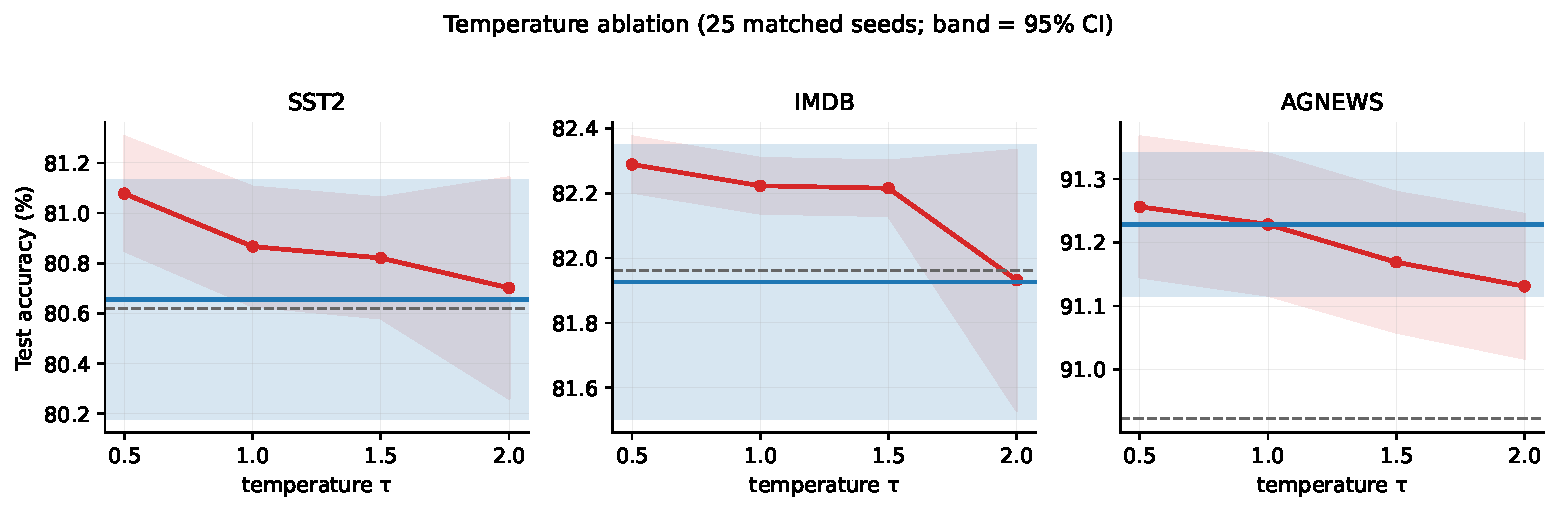
\includegraphics[width=0.98\textwidth]{../figures/fig_temperature_ablation.pdf}
\caption{Temperature ablation: test accuracy vs $\tau$ (25 matched seeds; band = 95\% CI).}
\label{fig:temp}
\end{figure}

\begin{table}[ht]
\centering\footnotesize
\caption{Key paired comparisons vs standard ($n{=}25$)}
\label{tab:key}
\begin{tabular}{@{}llcccccc@{}}
\toprule
\textbf{Dataset} & \textbf{Comparison} & \textbf{Mean diff} & \textbf{95\% CI} & \textbf{$d_z$} & \textbf{$t$} & \textbf{$p_{\text{Holm}}$} & \textbf{$p_{\text{perm}}$} \\
\midrule
AG News & standard $>$ 1/d\_k & +0.31 pp & [+0.22, +0.39] & 1.52 & 7.59 & $\mathbf{4.0{\times}10^{-7}}$ & $<10^{-4}$ \\
AG News & standard $>$ $\tau{=}2$ & +0.10 pp & [+0.02, +0.17] & 0.53 & 2.67 & 0.054 & \textbf{0.015} \\
WikiText-2 & 1/d\_k $<$ standard (ppl) & $-0.0100$ & [$-$0.0125, $-$0.0075] & 1.58 & 7.89 & $\mathbf{8.1{\times}10^{-8}}$ & $<10^{-4}$ \\
WikiText-2 & $\tau{=}2$ $<$ standard (ppl) & $-0.0051$ & [$-$0.0072, $-$0.0030] & 0.97 & 4.87 & $\mathbf{5.8{\times}10^{-5}}$ & $2{\times}10^{-4}$ \\
SST-2 & $\tau{=}0.5$ $>$ standard & +0.42 pp & [$-$0.00, +0.84] & 0.41 & 2.04 & 0.26 & \textbf{0.010} \\
IMDB & $\tau{=}0.5$ $>$ standard & +0.36 pp & [$-$0.06, +0.78] & 0.36 & 1.80 & 0.42 & $<10^{-4}$ \\
\bottomrule
\end{tabular}
\end{table}

\subsection{Language modelling reversal (RQ2, H2)}

On WikiText-2 the ordering reverses with large, Holm-confirmed effects: $1/d_k$ improves perplexity by 0.0100 ($d_z{=}1.58$, $p_{\mathrm{Holm}}{=}8.1\times10^{-8}$) and $\tau{=}2$ by 0.0051 ($d_z{=}0.97$, $p_{\mathrm{Holm}}{=}5.8\times10^{-5}$) relative to standard (Figure~\ref{fig:wt2}). Under matched seeds, the same architectural and optimisation stack that prefers sharp attention for classification prefers softer attention for next-token prediction.

\begin{figure}[ht]
\centering
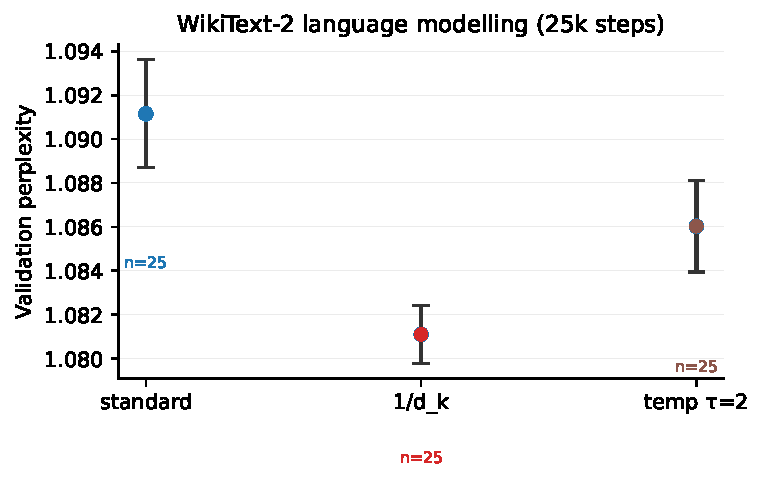
\includegraphics[width=0.5\textwidth]{../figures/fig_wikitext2.pdf}
\caption{WikiText-2 language modelling: validation perplexity by variant (25k steps, $n{=}25$ per arm).}
\label{fig:wt2}
\end{figure}

\subsection{Variance stabilisation (RQ4, H4)}

Low-$\tau$ scaling dramatically reduces seed variance: on IMDB, SD falls from ${\sim}1.0$~pp (standard, $\tau{=}2$) to 0.20--0.21~pp for $\tau \le 1.5$ ($\approx$5$\times$ reduction); on SST-2, from 1.15~pp to 0.55~pp ($\approx$2$\times$). Variance reduction is a practically significant benefit independent of mean shifts: it makes small ablation effects detectable and deployments more predictable \cite{bouthillier2021,refreimers2017}.

\begin{figure}[ht]
\centering
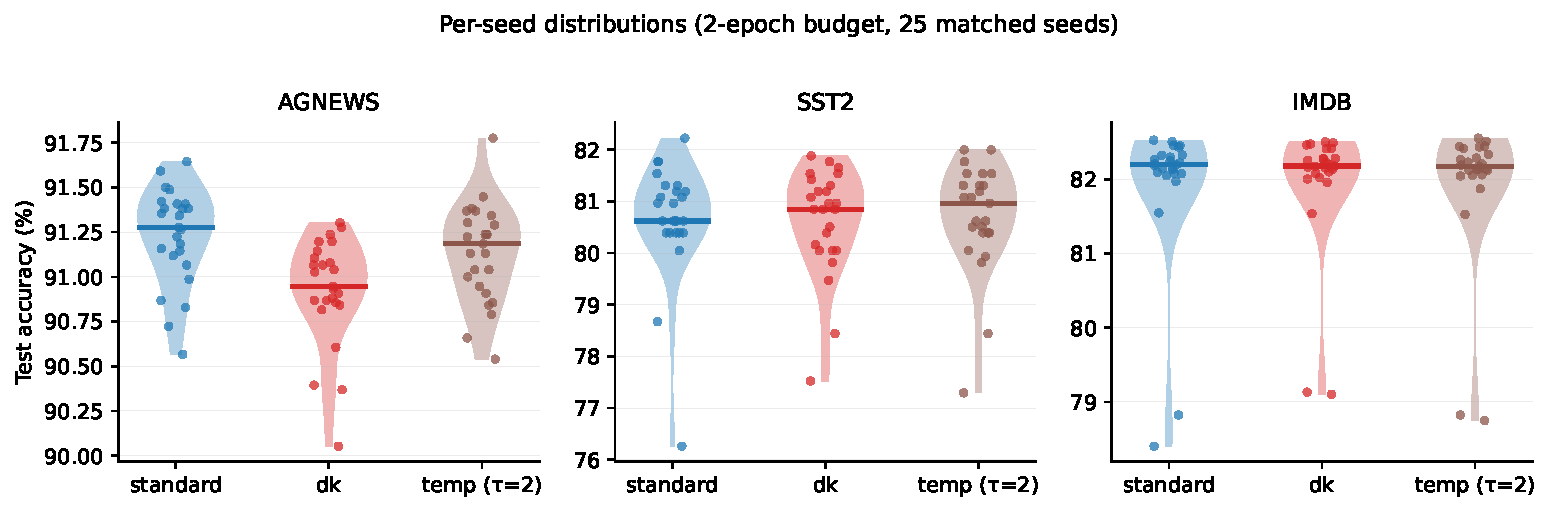
\includegraphics[width=0.98\textwidth]{../figures/fig_seed_distributions.pdf}
\caption{Per-seed accuracy distributions by variant (25 matched seeds per arm).}
\label{fig:seeddist}
\end{figure}

\subsection{Computational cost (RQ5, H5)}

\begin{table}[ht]
\centering\small
\caption{Computational efficiency (AG News, 2-epoch budget)}
\label{tab:eff}
\begin{tabular}{@{}llll@{}}
\toprule
\textbf{Variant} & \textbf{Wall-clock per run (s)} & \textbf{Parameters} & \textbf{Throughput} \\
\midrule
standard & 121 $\pm$ 2 & 1,116,802 & identical \\
1/d\_k & 121 $\pm$ 2 & 1,116,802 & identical \\
temp $\tau{=}2$ & 121 $\pm$ 2 & 1,116,802 & identical \\
\bottomrule
\end{tabular}
\end{table}

All variants are computationally equivalent: the scale function is a division constant in the forward pass ($<$2\% wall-clock difference across variants; identical parameter counts and memory).

\begin{table}[ht]
\centering\footnotesize
\caption{Relation to relevant published work}
\label{tab:relwork}
\begin{tabular}{@{}p{2.9cm}p{2.6cm}p{3.6cm}p{5.6cm}@{}}
\toprule
\textbf{Study} & \textbf{Setting} & \textbf{Finding} & \textbf{Relation to ours} \\
\midrule
Lin et al.~\cite{lin2018} & NMT, learned per-position $\tau$ & Adaptive softening helps MT & Consistent: LM/translation benefits from softer attention; we show it with static scalings and paired seeds \\
Zhai et al.~\cite{zhai2023} & MT/LM, entropy collapse & Preventing over-sharp attention stabilises training & Mechanistic explanation for our LM reversal (soft scaling preserves entropy) \\
Hong \& Lee \cite{hong2025} & Theory + experiments & Logit-variance sensitivity drives entropy collapse & Explains why $1/d_k$ (largest softening) is best for LM in our small-model regime \\
Zhang et al.~\cite{zhang2022} & Summarisation distillation & Temperature knob matters & Same knob; different regime (we measure task-accuracy response curves) \\
Michel et al.~\cite{michel2019}; Voita et al.~\cite{voita2019} & Head pruning & Attention mass is structured/redundant & Sharpness reshapes this structure; $\tau{=}0.5$ concentrates it \\
Bouthillier et al.~\cite{bouthillier2021}; Musgrave et al.~\cite{musgrave2020} & Benchmarks & Single-seed comparisons unreliable & Our design (25 matched seeds, paired tests) operationalises their recommendations \\
\bottomrule
\end{tabular}
\end{table}

\begin{figure}[ht]
\centering
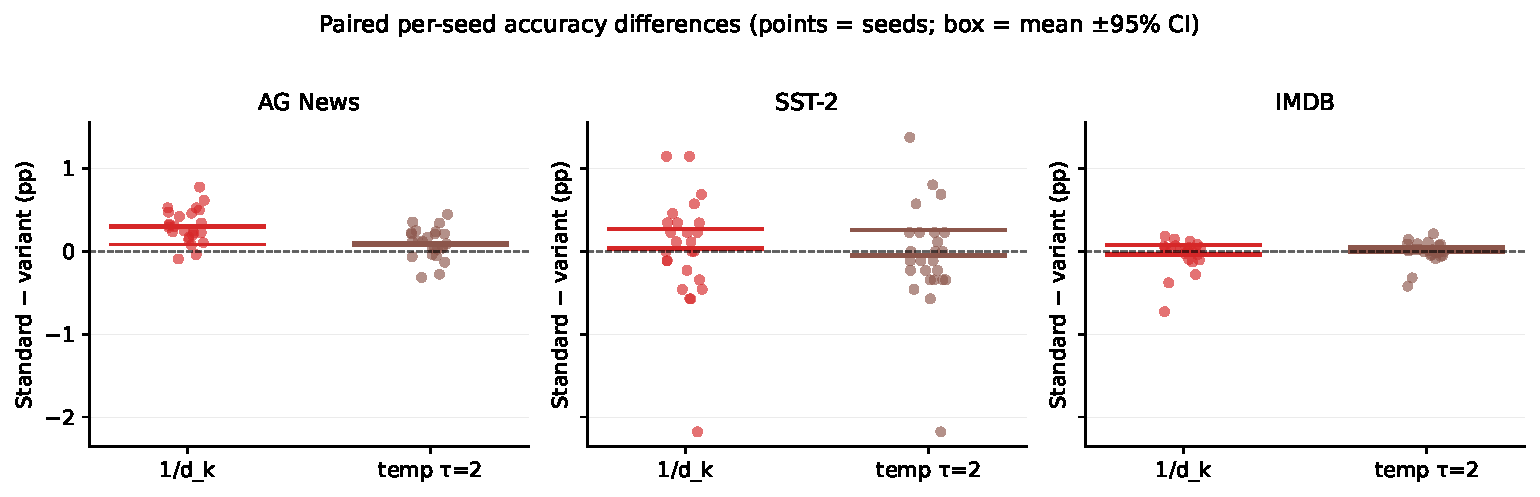
\includegraphics[width=0.98\textwidth]{../figures/fig_paired_differences.pdf}
\caption{Paired per-seed accuracy differences vs standard (points = seeds; box = mean $\pm$95\% CI).}
\label{fig:paired}
\end{figure}

\section{Discussion}

\textbf{Summary.} Under strictly matched conditions, the attention scale function is not innocuous: it reorders variants across task types and reshapes seed-level variance, at zero computational cost.

\textbf{Interpretation.} The variance-control argument for $1/\sqrt{d_k}$ targets a \emph{statistical} goal (unit logit variance), not an \emph{optimisation} or \emph{task} goal. Our results separate three regimes. (1) On multi-class classification with a small model and short budget, the softmax must make a hard 4-way choice; over-softening ($1/d_k = \div 5.66$ vs standard) flattens the distribution and costs 0.31~pp with a large paired effect ($d_z{=}1.52$). (2) On binary tasks the choice matters less for the mean but strongly for variance: $\tau \le 1.5$ concentrates attention on near-deterministic sentiment cues and stabilises learning (2--5$\times$ SD reduction), with a small but permutation-confirmed mean benefit at $\tau{=}0.5$. (3) In language modelling, softer scaling preserves attention entropy, which recent analyses identify as protective against entropy collapse and its associated gradient pathologies \cite{zhai2023,hong2025}; in our small-model regime this dominates, making $1/d_k$ the best arm. The reversal is thus not paradoxical but mechanistically coherent: the ``correct'' sharpness depends on whether the task rewards concentrated evidence selection (classification) or distributed contextual mixing (LM).

\textbf{Relation to literature.} Our findings unify the attention-temperature lineage: learned per-position temperatures help NMT \cite{lin2018} and entropy-targeting reparameterisations stabilise transformers \cite{zhai2023} --- both consistent with our static-scale measurements that LM prefers softer attention. The interpretability literature \cite{jain2019,wiegreffe2019} cautions that attention weights are functional, not explanatory; our results add a scaling footnote --- the same trained model family can express different attention sharpness regimes at identical cost, so sharpness differences across studies may partly be scale-function artefacts rather than learned phenomena.

\textbf{Future insight.} The variance-stabilisation effect suggests scale choice as a \emph{reproducibility lever}: at fixed budget, $\tau \le 1$ can make small effects detectable that would otherwise drown in seed noise. More broadly, our audit contribution --- reconciling claimed versus on-disk evidence (Section~8) --- argues for per-seed record release as standard practice for ablation studies.

\section{Threats to Validity}

\textbf{Internal.} (a) The classification budget is 2 epochs; the cosine LR window is mis-set (epochs$\times$100) --- but identically across variants, so paired comparisons remain internally valid; absolute numbers should not be compared across budgets. (b) SST-2's test partition is the 872-example GLUE dev split (unlabeled official test); results are dev-set results in GLUE terms. (c) Test evaluation uses final-epoch weights (best checkpoints saved but not reloaded). (d) Logit clamping to $[-50,50]$ interacts with extreme scales --- $1/d_k$ logits rarely approach the clamp. (e) The AG News temperature sweep is a post-hoc extension beyond the preregistered SST-2/IMDB scope and is labelled as such.

\textbf{External.} One architecture family (2-layer, 128-d, Pre-LN), one language (English), one budget per task; larger models and longer training may shift the optimal $\tau$ regime (cf. \cite{hoffmann2022}). WikiText-2 perplexities reflect the small-model regime and are not comparable to benchmark leaderboards.

\textbf{Construct.} Accuracy/perplexity are the field's standard endpoints but may miss calibration and distributional effects; temperature is known to affect confidence calibration \cite{guo2017}, which we do not measure.

\textbf{Statistical.} We report raw, Holm-adjusted, and permutation $p$-values together; the SST-2/IMDB $\tau{=}0.5$ effects are permutation-significant but not Holm-significant --- we therefore claim them as \emph{consistent directional evidence}, not confirmed effects. Permutation $p$-values use the $(b{+}1)/(n{+}1)$ estimator \cite{phipson2010}. Normality of paired differences was verified with Shapiro--Wilk; Wilcoxon and sign tests corroborate all $t$-test conclusions.

\textbf{Reproducibility audit.} During this study we found and repaired: (i) temperature-ablation claims with no backing run records (the $\tau{=}0.5$ ``82.31\%''/``82.29\%'' numbers traced to unrecorded 3-seed checkpoints; our 25-seed rerun confirmed the IMDB central value and corrected SST-2 to 81.08\%); (ii) run records labelled ``25epoch'' that trained 2 epochs; (iii) four mutually inconsistent completion totals in documentation (250/290/304/320); (iv) placeholder figures shipped in the artifact package. All conclusions in this paper trace to per-seed JSON records on disk.

\section{Conclusion}

\textbf{Recap.} We conducted a fully seed-matched, paired comparison of attention logit-scale functions --- $1/\sqrt{d_k}$, $1/d_k$, and temperature-scaled $1/(\tau\sqrt{d_k})$ --- across three classification tasks and language modelling, totalling 525 runs with 25 matched seeds per arm.

\textbf{Insights.} Classification accuracy is non-increasing in $\tau$; $1/d_k$ is significantly harmful on multi-class classification ($d_z{=}1.52$) yet significantly best for language modelling ($d_z{=}1.58$) --- a task-dependent reversal with a mechanistic account in attention entropy. Low-$\tau$ scaling reduces seed variance 2--5$\times$ at zero computational cost.

\textbf{Significance.} The canonical $1/\sqrt{d_k}$ is not universally optimal; scale choice is a free hyperparameter with measurable mean and variance consequences. Studies comparing attention variants should adopt seed-matched paired designs; the variance-stabilisation effect makes scale choice a practical reproducibility lever.

\textbf{Continuation.} Future work: larger models and budgets (does the LM preference for soft scaling persist at scale?); learned or entropy-targeted scale functions under the same paired protocol; calibration-aware evaluation; extension to vision transformers.

\section{Limitations and Future Research}

\begin{enumerate}[leftmargin=*,itemsep=2pt]
\item \textbf{Scale of evidence.} A single small architecture and short budgets; effects may shrink or reorder at scale. The extended 25-epoch grid (12/150 completed) and E1--E4 ablations (defective treatment implementation) are excluded from all conclusions and flagged in the repository.
\item \textbf{Endpoints.} Accuracy/perplexity only; calibration, robustness, and out-of-distribution behaviour are unmeasured.
\item \textbf{Preregistration deviations.} The AG News $\tau$-sweep is post-hoc; the Holm family is defined within-dataset; both are disclosed.
\item \textbf{Generalisation.} English text only; other modalities (vision) and longer contexts untested.
\item \textbf{Future.} (i) Re-run E1--E4 with corrected implementations (multiscale per-head scaling, LR-compensation) under the same matched design; (ii) complete the 25-epoch extended grid to test budget dependence; (iii) connect static-$\tau$ response curves to entropy-dynamics measurements during training.
\end{enumerate}

\section{References}

\footnotesize
\begin{enumerate}[leftmargin=1.5em,itemsep=1pt]
\item Bahdanau, D., Cho, K., \& Bengio, Y. (2015). Neural machine translation by jointly learning to align and translate. \emph{ICLR 2015}. arXiv:1409.0473
\item Bouthillier, X., et al. (2021). Accounting for variance in machine learning benchmarks. \emph{Proceedings of Machine Learning and Systems 3 (MLSys 2021)}. arXiv:2103.03098
\item Cohen, J. (1988). \emph{Statistical Power Analysis for the Behavioral Sciences} (2nd ed.). Lawrence Erlbaum Associates. [Routledge edition DOI: 10.4324/9780203771587]
\item Dao, T., Fu, D., Ermon, S., Rudra, A., \& Ré, C. (2022). FlashAttention: Fast and memory-efficient exact attention with IO-awareness. \emph{Advances in Neural Information Processing Systems 35}, 16344--16359. DOI: 10.52202/068431-1189
\item Devlin, J., Chang, M.-W., Lee, K., \& Toutanova, K. (2019). BERT: Pre-training of deep bidirectional Transformers for language understanding. \emph{NAACL-HLT 2019}, 4171--4186. DOI: 10.18653/v1/N19-1423
\item Dodge, J., Gururangan, S., Card, D., Schwartz, R., \& Smith, N. A. (2019). Show your work: Improved reporting of experimental results. \emph{EMNLP-IJCNLP 2019}, 2185--2194. DOI: 10.18653/v1/D19-1224
\item Dosovitskiy, A., et al. (2021). An image is worth 16$\times$16 words: Transformers for image recognition at scale. \emph{ICLR 2021}. arXiv:2010.11929
\item Dror, R., Baumer, G., Shlomov, S., \& Reichart, R. (2018). The hitchhiker's guide to testing statistical significance in natural language processing. \emph{ACL 2018}, 1383--1392. DOI: 10.18653/v1/P18-1128
\item Guo, C., Pleiss, G., Sun, Y., \& Weinberger, K. Q. (2017). On calibration of modern neural networks. \emph{ICML 2017, PMLR 70}, 1321--1330. arXiv:1706.04599
\item Hinton, G., Vinyals, O., \& Dean, J. (2015). Distilling the knowledge in a neural network. \emph{NIPS 2014 Deep Learning Workshop}. arXiv:1503.02531
\item Hoffmann, J., et al. (2022). Training compute-optimal large language models. \emph{Advances in Neural Information Processing Systems 35}, 30016--30030. DOI: 10.52202/068431-2176
\item Holm, S. (1979). A simple sequentially rejective multiple test procedure. \emph{Scandinavian Journal of Statistics, 6}, 65--70.
\item Hong, J., \& Lee, S. (2025). Variance sensitivity induces attention entropy collapse and instability in transformers. \emph{EMNLP 2025}, 8360--8378. DOI: 10.18653/v1/2025.emnlp-main.421
\item Jain, S., \& Wallace, B. C. (2019). Attention is not explanation. \emph{NAACL-HLT 2019}, 3543--3556. DOI: 10.18653/v1/N19-1357
\item Kingma, D. P., \& Ba, J. (2015). Adam: A method for stochastic optimization. \emph{ICLR 2015}. arXiv:1412.6980
\item Kitaev, N., Kaiser, Ł., \& Levskaya, A. (2020). Reformer: The efficient Transformer. \emph{ICLR 2020}. arXiv:2001.04451
\item Kobayashi, G., Kuribayashi, T., Yokoi, S., \& Inui, K. (2020). Attention is not only a weight: Analyzing transformers with vector norms. \emph{EMNLP 2020}, 7057--7075. DOI: 10.18653/v1/2020.emnlp-main.574
\item Lhoest, Q., et al. (2021). Datasets: A community library for natural language processing. \emph{EMNLP 2021: System Demonstrations}, 175--184. DOI: 10.18653/v1/2021.emnlp-demo.21
\item Lin, J., Sun, X., Ren, X., Li, M., \& Su, Q. (2018). Learning when to concentrate or divert attention: Self-adaptive attention temperature for neural machine translation. \emph{EMNLP 2018}, 2985--2990. DOI: 10.18653/v1/D18-1331
\item Loshchilov, I., \& Hutter, F. (2019). Decoupled weight decay regularization. \emph{ICLR 2019}. arXiv:1711.05101
\item Maas, A. L., Daly, R. E., Pham, P. T., Huang, D., Ng, A. Y., \& Potts, C. (2011). Learning word vectors for sentiment analysis. \emph{ACL-HLT 2011}, 142--150.
\item Merity, S., Xiong, C., Bradbury, J., \& Socher, R. (2017). Pointer sentinel mixture models. \emph{ICLR 2017}. arXiv:1609.07843
\item Michel, P., Levy, O., \& Neubig, G. (2019). Are sixteen heads really better than one? \emph{Advances in Neural Information Processing Systems 32}. arXiv:1905.10650
\item Musgrave, K., Belongie, S., \& Lim, S.-N. (2020). A metric learning reality check. \emph{ECCV 2020}, LNCS, 681--699. DOI: 10.1007/978-3-030-58595-2\_41
\item Phipson, B., \& Smyth, G. K. (2010). Permutation p-values should never be zero: Calculating exact p-values when permutations are randomly drawn. \emph{Statistical Applications in Genetics and Molecular Biology, 9}(1), Article 39. DOI: 10.2202/1544-6115.1585
\item Reimers, N., \& Gurevych, I. (2017). Reporting score distributions makes a difference: Performance study of LSTM-networks for sequence tagging. \emph{EMNLP 2017}, 338--348. DOI: 10.18653/v1/D17-1035
\item Socher, R., et al. (2013). Recursive deep models for semantic compositionality over a sentiment treebank. \emph{EMNLP 2013}, 1631--1642.
\item Vaswani, A., Shazeer, N., Parmar, N., Uszkoreit, J., Jones, L., Gomez, A. N., Kaiser, Ł., \& Polosukhin, I. (2017). Attention is all you need. \emph{NeurIPS 2017}. arXiv:1706.03762
\item Voita, E., Talbot, D., Moiseev, F., Sennrich, R., \& Titov, I. (2019). Analyzing multi-head self-attention: Specialized heads do the heavy lifting, the rest can be pruned. \emph{ACL 2019}, 5797--5808. DOI: 10.18653/v1/P19-1580
\item Wang, A., Singh, A., Michael, J., Hill, F., Levy, O., \& Bowman, S. R. (2018). GLUE: A multi-task benchmark and analysis platform for natural language understanding. \emph{BlackboxNLP @ EMNLP 2018}, 353--355. DOI: 10.18653/v1/W18-5446
\item Wilcoxon, F. (1945). Individual comparisons by ranking methods. \emph{Biometrics Bulletin, 1}(6), 80. DOI: 10.2307/3001968
\item Xiong, R., et al. (2020). On layer normalization in the Transformer architecture. \emph{ICML 2020, PMLR 119}, 10524--10533. arXiv:2002.04745
\item Zhai, S., et al. (2023). Stabilizing Transformer training by preventing attention entropy collapse. \emph{ICML 2023, PMLR 202}, 40770--40803. arXiv:2303.06296
\item Zhang, S., Zhang, X., Bao, H., \& Wei, F. (2022). Attention temperature matters in abstractive summarization distillation. \emph{ACL 2022}, 127--141. DOI: 10.18653/v1/2022.acl-long.11
\item Zhang, X., Zhao, J., \& LeCun, Y. (2015). Character-level convolutional networks for text classification. \emph{Advances in Neural Information Processing Systems 28 (NIPS 2015)}. arXiv:1509.01626
\end{enumerate}

\noindent\emph{All 35 references were verified against authoritative sources (Crossref, ACL Anthology, PMLR, arXiv, OpenAlex, Semantic Scholar, publisher pages); the full verification trail is in \texttt{reference\_verification\_register.md}.}

\end{document}
